%?? New angle -- \emph{Guarded} offers substantal improvements for \emph{most} internet traffic according to the stats we know. Is accurate protection of beningn UDP traffic actually more difficult?

%Talk about flaws here, what could go wrong...

%?? Why does SPF only do well sometimes? Model is actually more difficult to learn, so it seems to do best when it has a larger set of decisions to learn from. But, it does worse for TCP?
\fakepara{Model performance}
Of the results presented, \emph{Guarded}'s unpredictable (often worse) starting performance is unexpected, given its far smaller action space.
It's natural to expect that this would make the model easier to learn, but the additional state required appears to make the task \emph{harder}, beyond even the value of choosing a non-zero discount factor (adding forward-planning to explicitly mitigate this effect).
Accordingly, we see that this design performs best (and exhibits considerably lower variance) when agents learn from as much knowledge as possible: high $n$ and single-agent training.
To filter incoming traffic from a source, it must decide to degrade inbound traffic multiple times in a row, reducing the likelihood that a legitimate flow is punished by accident.
Our belief is that \emph{Guarded} is a considerably stronger model for these reasons, and its successes offer strong rationale to consider the best schemes for efficient information sharing.
Paradoxically, \emph{Instant} generally achieves the best performance for UDP traffic yet actively suffers when trained as a single learner---this may occur due to a roughly even spread of values between disparate actions, due to shared characteristics between legitimate and malicious flows.

%?? May be hard to learn multiple features at once while controlling multiple flows while contending with many more agents, with harder dynamics like TCP. Does this hinder learning in the long run?
Although we have improved upon Marl in both identified problem cases, the improvements are not quite on the order we'd expect for UDP traffic.
%?? I don’t know if you want to also mention the problem of things getting “stuck” in locally optimal (but globally sub-optimal) policies. I think it’s fairly uncontroversial that an increase in state space would make this more likely. Also, the lack of discounting could play a large role (and more so as the state space becomes more complex…
The most likely explanation is that agents are converging to, and becoming stuck in, locally optimal (but globally sub-optimal) policies.
The increased state space size makes this a more likely occurrence, as does the unclear effect of hyperparameters ($\alpha$, $\gamma$) as we scale up the state space.
We suspect that these difficulties may be exacerbated by the competitive nature of learning that these models embody: agents are learning action values for multiple features simultaneously, taking many actions at once (making it harder to observe the true value of each action), and controlling shared global state.
Although our design does take steps to counteract such effects, these mitigations may not be enough.
Moreover, benign UDP traffic shares many characteristics with attack traffic, suggesting that more training samples or some unknown feature might aid control, or that it may be worthwhile to extensively pre-train agents non-competitively on each feature using individual flows.

%It is likely that the design of Marl++ 
%?? Need to mention that Marl performs lower than their paper's numbers for TCP...

%Finally, it is crucial to note that the models and techniques presented here are an improvement , this work still trails behind existing (exact) DDoS flow detection mechanisms.
Most importantly, what we wish to impart is the knowledge that while the models and techniques we present here are a significant improvement over past RL-based work, this strand still trails behind existing (exact) DDoS flow detection mechanisms where TCP traffic is concerned.
The ability to better protect VoIP traffic when compared against one of these approaches is a curious observation, which suggests that other (exact) protocol-agnostic approaches may carry hidden assumptions and is a promising direction for future investigation.
Similar traffic makes up a significant fraction of network load today (\SIrange{18}{27}{\percent}).
Although we have conducted work to map the territory, there are still more advancements to be made before RL-based DDoS defence is truly competitive.
The benefits we have at present are, however, substantial.
What we offer above many of the approaches we discuss in \cref{sec:related-work} are potentially more flexible deployments, low-overhead and fixed-cost decision-making, without requiring active measurement or the network resources and capabilities that the most effective techniques rely upon.
Moreover, our decision making processes are entirely agnostic of the protocol or content of traffic, offering future-proofing against the introduction of new transports.

\fakepara{Security concerns and vulnerability}
Can an agent be flooded with new flows to reduce their ability to make decisions?
One of the risks introduced by our policy update strategy is that so much work can be queued up that an agent is never able to act on some attack flows.
The natural solution is to impose an upper bound on the amount of action computations/policy updates that can be performed before a work list is discarded completely.
This removes the guarantee that all flows will be visited fairly often, but if updates occur regularly then this random sampling may be sufficient to achieve good performance.

Can an attack on the controller can impact our approach?
This question hinges upon whether the deployment environment is a traditional network or is fully SDN-enabled---each agent is, in a sense, \emph{a} controller alongside the network's controller.
In a traditional network, only the agents act as controllers, but since they periodically request per-flow data (rather than continuously receiving it) no amount of flows generates more requests or messages to the agent.
More work is generated, but we discuss how to handle this safely above.
Accordingly, agents can never be stalled by request volume: their only remote communication (load measurements) comes from trusted nodes, is highly periodic, and has constant size.
The same logic holds for a fully software-defined network.
Recalling that we do not employ the network's controller to install filtering rules on edge switches, an agent's ability to act is unimpeded.
Thus, the controller is made no more vulnerable than in any other SDN.
The only necessary change for such a scenario is that a load measurement which has not been updated (due to a timeout or missed deadline) should be set at $R_t=-1$.
%\begin{figure}
%	\centering
%	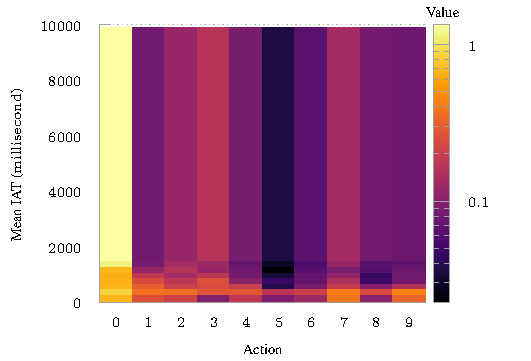
\includegraphics[width=0.9\linewidth]{../plots/policy-16-tcp-f5-mean-log}
%	
%	\caption{
%		Mean Marl action values from pre-training on mean IATs ($n=16$).
%		As these are mean values, lighter cells in each row indicate actions \emph{likely} to be taken by an agent's policy.
%		Repeated values originate from the bias tile, which is always active, and indicate regions of the state-space which have yet to be visited---here, this is most of the state space.
%		Agents visibly learn action values for tiles which override the default bias tile's preferences.
%		The measured effectiveness of this feature then suggests that a low-resolution coding over the standard region may, in fact, be a better choice.
%		We see that agents prefer to choose $p=0.0$ in most states, but higher $p$ when IATs are particularly small.
%		\label{fig:intern-16-tcp-iat}
%	}
%\end{figure}
%
%\begin{figure}
%	\centering
%	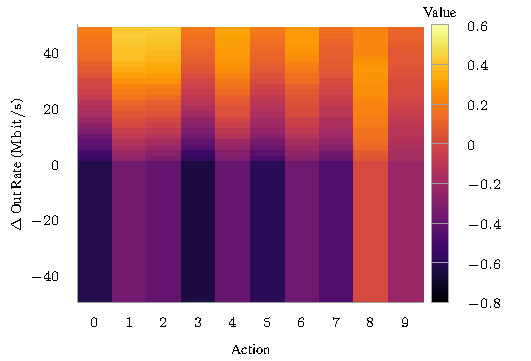
\includegraphics[width=0.9\linewidth]{../plots/policy-4-tcp-f7-mean}
%	
%	\caption{
%		Mean Marl action values from pre-training on $\Delta$ out rates ($n=4$).
%		A sudden ramp-up of server-to-host traffic is used as a strong indicator of flow legitimacy, while more punishing actions have comparatively higher value as $\Delta$ out rate decreases.
%		Furthermore, we see again that a region of the state space has gone somewhat unexplored---we observed after plotting this visualisation that many decreases in this feature are too small to hit the adjacent tile, which implies a mixed-resolution coding may improve an agent's policy further.
%		\label{fig:intern-16-tcp-something}
%	}
%\end{figure}

%?? Is the state space interpretable? Yes!
Machine learning algorithms have earned a reputation for eluding human interpretation, while being vulnerable to evasion and poisoning.
Given the security risks associated with introducing such techniques, it is natural to be concerned with the interpretability of the models we have proposed.
With the exception of global state, the tile coding parameters we make use of ensure that the set of outputs for each feature we add is relatively enumerable: for $n$ tilings and $c$ tiles per dimension there are $nc^{\dim{f}}$ individual action value vectors per feature $f$ (\num{48} for the new features we introduce, \num{10368} for global state), though considerably more combinations thereof ($c^{n \cdot \dim{f}}$).
%\Cref{fig:intern-16-tcp-iat,fig:intern-16-tcp-something} show how we may visualise the portion of a policy for each feature, and describe what information can be gained from doing so.
Furthermore, system state which is dependent on many signals drawn from across a wide network (such as our global state) is difficult to exert precise control over.
These signals' topological separation, in concert with their burstiness and unpredictability, may have substantial effects on an attacker's capabilities.

\fakepara{Real-world Deployment}
Currently, we assume that switches support an extension to OpenFlow to enable remotely installable packet-drop rules, either by running a modified version of OVS on commodity hardware at these locations or through custom firmware for egress switches.
Similar functionality could be employed by making use of OpenFlow's meter rules.

Where overheads are concerned, the state space sizes guarantee that an \emph{Instant} agent's policy remains under \SI{520}{\kibi\byte}, although in practice our sparse representation typically leads to far smaller policies: $\sim$\SI{17.8}{\kibi\byte} from our experiments.
\emph{Guarded} policies are \SI{30}{\percent} of this size.
As we have described earlier, action updates require a constant number of floating point operations---\num{160} floating point additions and \num{32} multiplications per update of $\wvec{}$ with per-tile updates, above the \num{160} additions required to choose an action.
The vast majority of these operations can be vectorised trivially, if such hardware is present.
Action computation for \emph{Guarded} agents is cheaper still, requiring only \num{48} additions per action.
Beyond this, we require that egress switches are capable of co-hosting an agent (i.e., through \emph{network function virtualisation}), with the necessary hardware to support this.
We believe that it may be possible to implement similar behaviour on standard commodity switches through application of \emph{programmable data planes} \cite{DBLP:conf/ancs/JouetP17}.

%?? Incorrect, pickling...
%?? deployment/system guidelines, architecture, and overhead/footprint of doing this
%?? Mention: probably fewer state measurements than in our emulations, but longer measurements means less noisy (so probably more accurate)
Gathering and transmission of load/flow statistics would be difficult to perform as often as an emulated environment allows, without inadvertently affecting host traffic.
However, the measurements acquired in such a scenario are likely to be less noisy (by being collected over longer periods of time), which could aid training.
The main bottlenecks are likely in forwarding the load measurements from various aggregation points (which can be made more efficient through multicast) and in running some estimator $\operatorname{g}(\cdot)$ to condition the reward function.
%?? Potential for dividing up pre-feature training across different agents, or train like this locally (sets of flows trained by 1 sub-model).
%?? Different global state per-agent? Seems this must be locally trained, just make it (everything up the chain to key destinations).
We expect that agents will be able to share policies for all features, which may help to offset the reduced rate of incoming experience.
Regardless, it will take longer to achieve enough state-state transitions to converge on a good policy.

One limit of SDN-capable hardware is that OpenFlow rules occupy \SI{6}{$\! \times$} the space of standard rules---commercial switches only have TCAM space for \numrange{2000}{20000} rules \cite{DBLP:journals/comsur/NguyenSBT16}.
Our approach consumes a rule for each active flow (the host density), and by the end of an experiment a switch can accrue around \num{900} rules.
While we use a default fallback action to maintain connectivity, eviction of high-value decisions which filter high-bandwidth attackers poses a significant risk.
Given that most flows are small (with the majority of bytes coming from a few ``heavy-hitters'') \cite{DBLP:journals/ccr/PanBPS03}, it may suffice to only apply RL-based analysis to larger flows.
%?? What could we do in the meantime? I propose manually assigning elephant flows a high importance rule, while increasing the importance of "block" decisions even higher.
OpenFlow rules have an \emph{importance}, controlling which rules may be evicted by a new entry (preventing entries from evicting those with higher importance).
If an agent is to act on all flows, a solution is to assign an importance of 0 to mice flows, 1 to elephant flows, and 2 to total filtering (leaving agents to time out and remove elephant flow rules to prevent bloat).
Given the high churn and prevalence of mice flows, eviction here is most likely to affect flows which are complete.
In both cases, extra rules can be made available by upgrading rules which completely filter a flow into upstream blackholing (as in collaborative approaches \cite{DBLP:conf/acsac/RamanathanMYZ18}), having the agent remove this rule once blackholing is active.